\section{Bandit Approach Results} 

\subsection{Copeland Scores}

The five subjects in the study preferred four different parameter sets out of
the nine parameter sets they could choose from, thereby demonstrating that the
offline optimization approach can generate parameters that suit different users.
\Cref{fig:copeland} shows the total Copeland score achieved by each parameter
set across all five subjects. From this chart, we can see it is possible, as in
the case of parameter set 6, that a controller receives high scores from some
users while receiving a score of zero from other users. This illustrates the
importance of tailoring prostheses to individual users. Some parameters such as
parameters 1, 4, and 8, achieved consistently low scores across all users. It
may be possible for us to remove these parameters from future studies. However,
more subjects would be needed before making such a determination as parameter
set four received a relatively high score from subject five.

\begin{figure}[b]
    \centering
    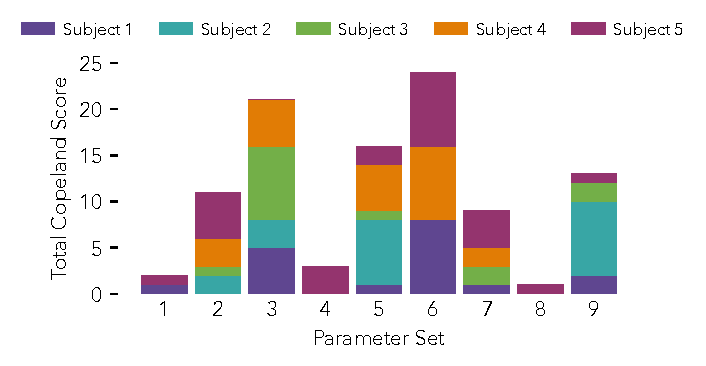
\includegraphics[width=\columnwidth]{copeland_scores_new}
    \caption{Total Copeland score achieved by each parameter set across all five
    subjects.}\label{fig:copeland}
\end{figure}

\begin{figure}[t]
    \centering
    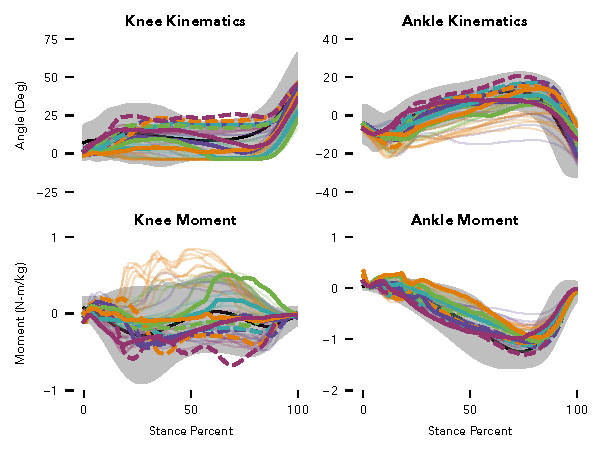
\includegraphics[width=\columnwidth]{kin_all_arms}
    \caption{Median angles and moments at \unitfrac[0.8]{m}{s} for all parameter
    sets for all subjects. Thicker weight solid lines indicate each subject's
    gait with their preferred parameters. Dashed lines indicate gait with
    hand-tuned parameters. The grey shaded regions show the mean and three sigma
    intact subject gait data (from the extra slow walking data in
    \citep{bovi2011multiple}).}\label{fig:kin_all_arms} 
    \vspace{-0.3cm}
\end{figure}

\subsection{Kinematics and Kinetics at \unitfrac[0.8]{m}{s}}
\Cref{fig:kin_all_arms} shows the ankle and knee kinematics achieved by all
subjects on all parameters at \unitfrac[0.8]{m}{s}. The thicker solid lines
indicate the gait data produced by subjects' preferred parameters and the dashed
lines indicate the gait data produced by the hand-tuned parameters. We see that
subject gait with both their preferred parameters and hand-tuned parameters
follow similar trends to intact gait data~\citep{bovi2011multiple}, whose mean
and three sigma variance is shown as the blue shaded region. However, all
subjects preferred the optimized parameters to the hand-tuned set. 

Just as in the intact data, there is significant variation in subjects'
preferred gait characteristics, which reinforces the idea that targeting a
specific kinematic or kinetic pattern may not be ideal for all users. This seems
to be especially true of the knee joint moment, where there are significant
differences in the amount of knee extension torque in early stance and flexion
torque in late stance among users. 

We found that most subjects produced relatively little ankle dorsiflexion as
they walked. Consequently, for most subjects the neuromuscular model control
produced less ankle plantarflexion torque than is average for able-bodied
subjects.  We believe the low level of ankle dorsiflexion was caused by the
relatively short foot of the prosthesis, which we plan to rectify for future
experiments. However, this effect also betrays a potential weakness of the
approach: optimizing to match able-bodied kinetics given able-bodied kinematics
may not be able to rectify some types of discrepancies between the human and
the prosthesis.

\subsection{Control Performance at Higher Gait Speeds}
\begin{figure}
    \centering
    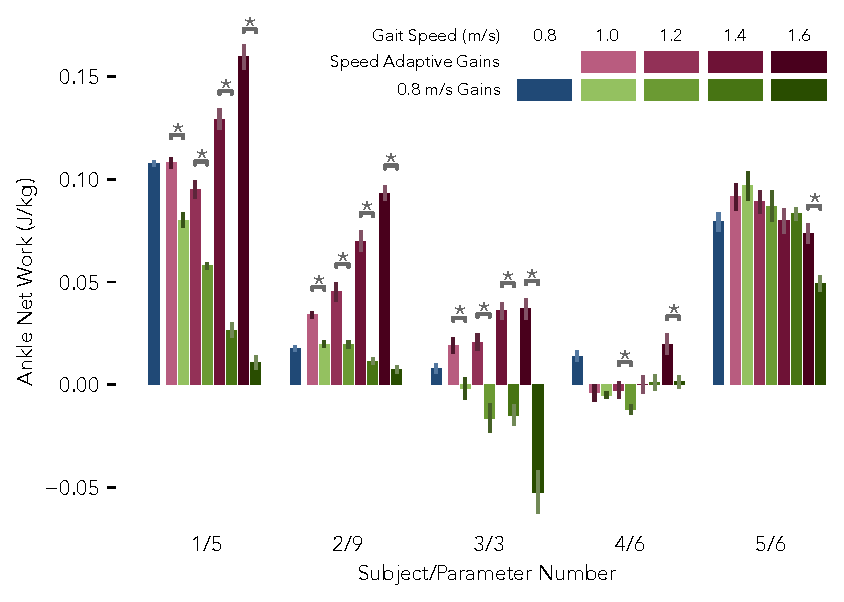
\includegraphics[width=\columnwidth]{net_work_vs_speed_new_annotated}
    \caption{Average net ankle work for each subject at each speed. Purple bars
    indicate trials where speed-adaptive gains were used whereas green bars
    indicate trials performed with the gains for \unitfrac[0.8]{m}{s}. Stars
    indicate statistically significant differences between the work produced by
    the speed adaptive gains and that produced by the \unitfrac[0.8]{m}{s} gains
    $(p < 0.05)$.}\label{fig:net_work_vs_speed}
\end{figure}

\Cref{fig:net_work_vs_speed} shows the average net ankle work\footnote{The area
within the torque versus angle plot of the ankle over a stride.} produced by the
control strategy at speeds ranging from \unitfrac[0.8 to 1.6]{m}{s}. Data from
subjects 1, 2, and 3, who chose parameter sets 5, 9, and 3 respectively, show a
clear downwards trend in ankle work as speed increases when using a constant set
of gains. On the other hand, with the adaptive gains, as speed increases ankle
work increases, mimicking the behavior of the biological ankle
\citep{herr2012bionic}. All three of these subjects preferred the behavior of
the adapted parameters to the parameters for \unitfrac[0.8]{m}{s} when walking
at \unitfrac[1.4 and 1.6]{m}{s}.

Subjects 4 and 5 both chose parameter set six and show no clear trend in ankle
work as speed increases. For this parameter set, the speed adapted gains only
increased ankle work significantly over baseline at \unitfrac[1.6]{m}{s} for
both subjects. Additionally, these two subjects indicated no trend in
preference between the adapted and unadapted parameters at the higher speeds.
These two subjects produced different amounts of net work despite using the same
parameter set. This is likely due to kinematic differences between the subjects
as well as differently tuned bias settings for the ankle joint.

From this result we can conclude that the offline optimization approach can
produce improved responses at speeds other than that at which we conduct the
online optimization, but that the improvement needs to be confirmed on a
per-parameter basis. It is not currently clear why parameter set six does not
exhibit increasing ankle work as speed increases as the underpinning human data
for this parameter set does indeed exhibit the desired trend. The issue could
possibly lie with the structure of the high level control or with local minimums
obtained by the CMA-ES method. 
